
\documentclass[12pt,aspectratio=169]{beamer}
\usepackage{xcolor}
\usepackage{hyperref}

\usetheme{default}

\setbeamercovered{invisible}
\setbeamertemplate{navigation symbols}{}
\setbeamertemplate{footline}{
    \flushright{\hfill \insertframenumber{}/\inserttotalframenumber}
}


\begin{document}
  \title{Lab01 - Compiling}
  \author{Matteo Caldana}
  \date{28/09/2023}
    
  \begin{frame}[plain, noframenumbering]
    \maketitle
  \end{frame}

\begin{frame}{Code organization}

  A typical C++ program is organised in {\color{blue} header} and {\color{blue} source} files.  
  \smallskip

  \alert{Header files} contains the information that
  describes the public interface of your code: declarations,
  definition of function class templates, etc. 
  C++ header files have (normally) extension \texttt{.hpp} and are eventually stored in special directories with name \texttt{include}.
  \smallskip

  \alert{Source files} contain the implementations (definitions of variables/functions/methods) and are normally collected
  under the directory \texttt{src}. Only one source files contains the \texttt{main()} program.
  \smallskip

  {\color{blue} Libraries} can be static or dynamic (shared). For the moment let's think the library as a
  collection of compiled files that can be used (linked) by an external
  program. 
  \smallskip

  
\end{frame}

\begin{frame}{Template libraries}

  {\color{blue} Template libraries} are a special case that consists only of header files, so go in \texttt{include/}. Since they are not pre-compiled this makes life much simpler, but compilation time longer. A template function is not \textit{real code} until it is \textit{specialized} (used).

  \centerline{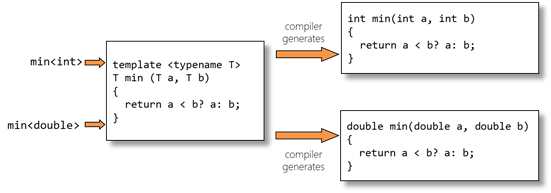
\includegraphics[width=0.85\textwidth]{template}}
   
\end{frame}


\begin{frame}{Why the separation into header and source?}

The reason is that all source files that uses an item (they call a function for example) need to see the \alert{declaration} of the item in order to compile. This is done by \alert{including} the header file containing the declarations.
Only one source file will provide the \alert{definition} of the item: it's the source file whose compilation will produce the actual machine code for that item. Indeed, you cannot have \alert{more than one definition} (one definition rule, also called odr.)
\medskip

Remember however that \alert{a definition is also a declaration}.
 
\end{frame}

\begin{frame}[fragile]
\frametitle{Translation unit}
A C++ \alert{translation unit} (also called compilation unit) is formed by a \alert{source file}  and all the (recursively) \texttt{include}d header files it contains.

A program is normally formed by more translation units, one and only one of which is the \alert{main program}.
\medskip

The important concept to be understood is that during the compilation process \alert{each translation unit is treated separately} until the last step (linking stage).

\end{frame}

\begin{frame}{The compilation steps (simplified)}
Compiling an executable is in fact a \alert{multistage process} formed by different components. The main ones are
\begin{itemize}
	\item \alert{Preprocessing}. Each translation unit is transformed into an intermediate source by processing C++ directives (\texttt{-E} flag);
	\item \alert{Compilation} proper. Each preprocessed translation unit is converted into an {\color{blue} object file} (\texttt{-c} flag). Most optimization is done at this stage;
	\item \alert{Linking} Object files are assembled and unresolved symbols resolved, eventually by linking external libraries, and an executable is produced.
\end{itemize}

When you launch the executable, you have an additional step:
\begin{itemize}
	\item \alert{Loading} Possible dynamic (shared) library are loaded to complete the linking process. The program is then loaded in memory for execution. 
\end{itemize}
\end{frame}

\begin{frame}{The compilation steps (simplified)}
  \centerline{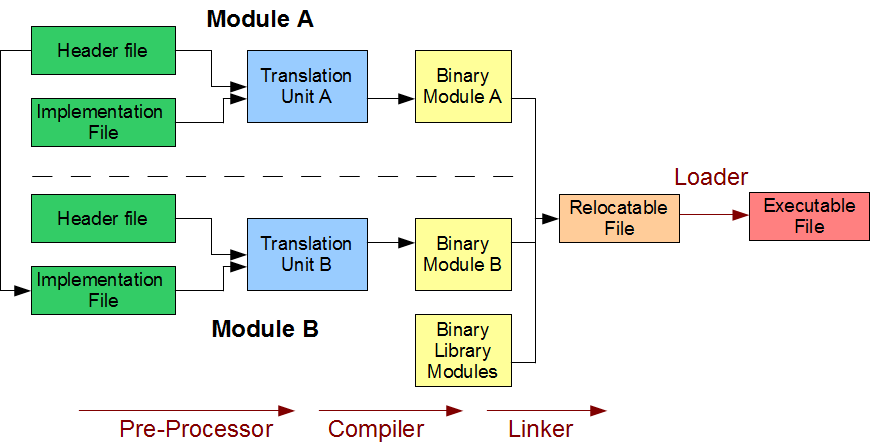
\includegraphics[width=0.99\textwidth]{compile_steps}}
\end{frame}


\frame{
\frametitle{What should a header file contain}
{\small
\begin{center}
\begin{tabular}{ll}
\alert{Named namespaces} & namespace LinearAlgebra\\
\alert{Type declarations} & class Matrix\{...\}\\
\alert{Extern variables declatations} & extern double a;\\
\alert{Constant variables}&const double pi=4*atan(1.0) \\
\alert{Constant expressions}&constexpr double h=2.1 \\
\alert{Constexpr functions}&constexpr double fun(double x)\{...\}\\
\alert{Enumerations} & enum bctype \{...\}\\
\alert{Function declarations} & double norm(...);\\
\alert{Forward declarations} & class Matrix;\\
\alert{Includes} & \#include\texttt{<iostream>}\\
\alert{Preprocessor directives} & \#ifdef AAA\\
\alert{Template functions} & template \texttt{<class T>} fun(T x)\{...\};\\ 
\alert{Inline functions} & inline fun()\{...\}\\
\alert{constexpr functions} & constexpr fun()\{...\}\\
\alert{automatic functions} & auto fun(auto x)\{...\}\\
\alert{type alias} & using Real=double;
\end{tabular}
\end{center}
}
}

\frame{
\frametitle{\alert{What a header file should not contain}}
{\small
\begin{center}
\begin{tabular}{ll}
\alert{Function definitions}\footnote{unless inline, constexpr functions or template functions} & double norm()\alert{\{ ..\}}\\
\alert{Method definitions} & double Mat::norm()\alert{\{ ..\}}\\
\alert{Definition of non-constexpr variables}& double bb=0.5;\\
\alert{Definition of static class members}& double A::b;\\
\alert{C array definitions} & int aa[3]=\{1,2,3\};\\
\alert{Array definitions} & std::array$<$double,3$>$ a\{1,2,3\};\\
\alert{Unnamed namespaces}&namespace \{ ...\} \\
\end{tabular}
\medskip


\end{center}
}
}


\frame
{
\frametitle{Useful flags}

{\small
Command \alert{\texttt{g++ -std=c++17 -o prog prog.cc}} would execute both
\emph{compilation} and \emph{linking} steps.

{\scriptsize
\begin{center}
MAIN  g++ OPTIONS (\textcolor{blue}{some are in fact preprocessor or linker options})
\smallskip

\begin{tabular}{ll|ll}
  -g & For debugging & -O[0-3] -Ofast & Optimization level\\
  -Wall, -Wextra & Activates  warnings & -I\texttt{dirname}& Directory of header files\\
  -D\texttt{MACRO} & Activate MACRO & -L\texttt{dirname} & Directory of libraries\\ 
  -o file          & output in file & -l\texttt{name}  & link library\\
  -std=c++14 &activates c++14 features &-std=c++20 &activates c++20 features\\
  -std=c++17 &activates c++17 features &-c &create only object file\\
  -S & output assembly code &-E &create only pre-processed files\\
  -v & verbose compile & -g & keep debugging symbols\\
\end{tabular}
\end{center}
The default C++ version for g++ versions 9 and 10 is \texttt{c++14}. In version 11 is \texttt{c++17}.
}}
}

\begin{frame}[fragile]
  \frametitle{The compilation process}
  But in fact the situation  is usually more complex, \alert{we normally have more than one translation units (source files)}

\begin{verbatim}
g++ -std=c++20 -c a.cpp b.cpp 
g++ -std=c++20 -c main.cpp
\end{verbatim}

  produce the \alert{object files} \texttt{a.o}, \texttt{b.o} and
  \texttt{main.o}. Only one of them contains the \alert{main program}
  (\texttt{int main(){...}}).

  Then,
\begin{verbatim}
g++ -std=c++20 -o main main.o a.o b.o
\end{verbatim}
  produces the \alert{executable} \texttt{main} (linking stage).
  \smallskip
  
  Each translation unit \alert{is compiled separately, even if they are
    in the same compiler command}.
\end{frame}

\begin{frame}[fragile]{All in one go}
	Of course it is possible to do all in one go
  \begin{verbatim}
  g++ -std=c++20 main.cpp a.cpp b.cpp -o main
  \end{verbatim}	
  But it is normally better to keep compilation and linking stages separate. If you modify \texttt{a.cpp} you have
  to recompile only \texttt{a.o} and repeat the linking.
  \smallskip

  Note however, that the compiler will in any case treat the translation units \texttt{a.cpp}, \texttt{b.cpp} and \texttt{main.cpp} separately.


  \medskip

  Let's look at the 3 stages in more detail.
\end{frame}

\begin{frame}
  \centering
  \Large
  \color{blue} Let's try this on a Hello World
\end{frame}
 
\frame{ \frametitle{The preprocessor} 

  To understand the mechanism of the header files correctly it is
  necessary to introduce the C preprocessor (\alert{\texttt{cpp}}).  It is
  launched at the beginning of the compilation process and it modifies
  the source file producing another source file (which is normally
  not shown) for the actual compilation.  \medskip


  The operations carried out by the preprocessor are guided by
  \alert{directives} characterized by the symbol \alert{\#} in the
  first column.  The operations are rather general, and the C
  preprocessor may be used non only for C or C++ programs but also for
  other languages like FORTRAN!. 

}


\frame{
\frametitle{The preprocessor}
Very rarely one calls the preprocessor explicitly, yet it may be
useful to have a look at what it produces

To do that one may use the option \texttt{-E} of the compiler:

\texttt{g++ -E [-DVAR1] [-DVAR2=xx] [-Iincdir] file >pfile}
\medskip

\alert{Note:} \texttt{-DXX} and \texttt{-I<dirname>} compiler options are in fact \textcolor{blue}{\textbf{cpp options}}.
\smallskip

The first indicates that the preprocessor \alert{macro variable}
\texttt{XX} is set, the second indicates a directory where the compiler may look for header files.
}


\frame{
\frametitle{Main  \texttt{cpp} directives}
All preprocessor directives start with a hash (\texttt{\#})  at the first column.
\smallskip


\begin{center}
\texttt{\#include<filename>}
\end{center}
Includes the content of  \texttt{filename}. The file is searched
fist in the directories possibly indicated with the option 
\texttt{-I\alert{dirname}}, then in the system directories (like \texttt{/usr/include}).
\smallskip

\begin{center}\texttt{\#include "filename"}\end{center}
Like before, but first the \alert{current directory} is searched for
\texttt{filename}, then those  indicated with the option 
\texttt{-I\alert{dir}}, then the system directories.
}

\frame{
\centerline{\texttt{\#define VAR}}

Defines the \emph{macro variable} \texttt{VAR}. For instance
\texttt{\#define DEBUG}. You can test if a variable is defined by
\texttt{\#ifdef VAR} (see later). The preprocessor option
\texttt{-DVAR} is equivalent to put {\texttt{\#define VAR}} at the
beginning of the file. Yet it \alert{overrides} the corresponding directive, if present.

\medskip

\centerline{\texttt{\#define VAR=nn}}

It assigns value \texttt{nn} to the (\emph{macro variable})
\texttt{VAR}.  \texttt{nn} is interpreted as an alphanumeric
string. Example: \texttt{\#define VAR=10}.  Not only the test
\texttt{\#ifdef VAR} is positive, but also \alert{any occurrence} of
\texttt{VAR} in the following text is replaced by \texttt{10}. The corresponding cpp option is \texttt{-DVAR=10}.
}

\frame{
\begin{ttfamily}
\begin{center}
\begin{flushleft}
\#ifdef VAR\\
\color{blue} code block \color{black} \newline
\#endif
\end{flushleft}
\end{center}
\end{ttfamily}

If \texttt{VAR} is {\color{red} undefined} \color{blue} code block \color{black} is
\alert{ignored}. Otherwise, it is output to the preprocessed source.
\medskip

\begin{ttfamily}
\begin{center}
\begin{flushleft}
\#ifndef VAR\\
\color{blue} code block \color{black} \newline
\#endif
\end{flushleft}
\end{center}
\end{ttfamily}


If \texttt{VAR} is {\color{red} defined}  \color{blue} code block \color{black} is
\alert{ignored}. Otherwise, it is output to the preprocessed source.
}

\begin{frame}[fragile]
\frametitle{Special macros}
The compiler set special macros depending on the options used, the programming language etc. Some of the macros are compiler dependent, other are rather standard:
\begin{itemize}
\item \texttt{\_\_cplusplus} It is set to a value if we are compiling with a
  c++ compiler. In particular, it is set to \texttt{201103L} if we are
  compiling with a C++11 compliant compiler.
\item \texttt{NDEBUG} is a macros that the user may set it with the \texttt{-DNDEBUG} option. It is
  used when compiling ``production'' code to signal that one {\color{blue}
    DOES NOT} intend to debug the program. It may change the behavior
  of some utilities, for instance \texttt{assert()} is deactivated if
  \texttt{NDEBUG} is set. Also some tests in the standard library algorithms are deactivated. Therefore, you have a more efficient program.
\end{itemize}

\end{frame}


\frame{
\frametitle{The header guard}
To avoid multiple inclusion of a header file the most common technique
is to use the {\color{blue} header guard}, which consists of checking if a
macro is defined and, if not, defining it!

\begin{semiverbatim}
\color{red} \#ifndef HH\_MYMAT0\_\_HH \newline
\#define HH\_MYMAT0\_\_HH\newline
\color{black}
... Here the actual content \newline
\color{red}
\#endif
\color{black}
\end{semiverbatim}

The variable after the \texttt{ifndef} (\texttt{HH\_MYMAT0\_\_HH} in the example) is chosen by the programmer. It should be a long name, so that it is very unlikely that the same name is used in another header file!

Some IDEs generate it for you!
}


\begin{frame}{The compilation proper}
After the preprocessing phase the translation unit is translated into an \texttt{object code}, typically stored in a file
with extension \texttt{.o}.
\medskip

{\color{blue} Object code, however, is not executable yet}. The executable is produced by gathering the functionalities contained in several object files (and/or libraries). 
\medskip

\begin{semiverbatim}
g++ -std=c++20 -c -Wall a.cpp b.cpp
\end{semiverbatim}
run preprocessig+compilation proper and produces the object files \texttt{a.o} and \texttt{b.o}.

\end{frame}

\begin{frame}{The linking process}
The process to create an executable from object files is done by calling the linker using \emph{the same name of the compiler used in the compilation process}.
\begin{semiverbatim}
g++ main.o a.o b.o -lmylib -o myprogram
\end{semiverbatim}
The linker is called with the same name of the compiler (\texttt{g++} in this case) so it knows which system libraries to search! Here, it will search the c++ standard library. If you call the standalone linker, called \texttt{ld} you need to specify yourself where the c++ standard library resides!
\smallskip

You have to indicate possible other libraries used by your code. In this case the library \texttt{libmylib}.
\end{frame}

\begin{frame}{Handle all this complexity}
  If all this complexity seems a little bit over bearing to you, do not worry, there are tools that help you automate the builds of large projects. Here a couple:
  \begin{itemize}
    \item The \alert{make} utility is a tool to produce files according to user
    defined, or predefine, rules. The rules are written on a file, usually called {\color{blue} Makefile}. See \url{https://makefiletutorial.com/}, \url{https://www.gnu.org/software/make/manual/make.html}.
    \item The \alert{CMake} is cross-platform software for build automation with support for many IDEs. It is easy to learn since it is a much higher level tool than make. See \url{https://cmake.org/}.
  \end{itemize}
\end{frame}


\begin{frame}{Back to libraries}
\alert{Static} libraries are the oldest and most basic way of integrating
``third party'' code. They are basically a collection of object file
stored in a single archive. 
At the linking stage of the compilation processes the symbols
(which identify objects used in the code) that are still unresolved
(i.e. they have not been defined in that translation unit) are
searched in the indicated libraries, and the corresponding code is
inserted in the executable.
\smallskip

With \alert{shared} libraries, the linker just makes sure that the symbols that are still
unresolved are indeed provided by the library, with no ambiguities.
But the corresponding code is not inserted, and the symbols
remains unresolved. Instead, a reference to the library is stored in
the executable for later use by the loader.
\end{frame}

\begin{frame}{Advantages and disadvantages of static libraries}
  \begin{center}
    \alert{PROS}
    \end{center}
    The resulting executable is \emph{self contained}, i.e. it contains all
    the instructions required for its execution.
    \begin{center}
    \alert{CONS}
    \end{center}
    \begin{itemize}
    \item To take advantage of an update of an external library we need to
      \alert{recompile the code} (at least to replicate the linking
      stage), so we need the availability of the source (or at least of the
      object files);
    \item We cannot load  symbols dynamically, on the base of decisions
      taken run-time (it's an advanced stuff, we will deal with it in another lecture);
    \item The executable may become large.
    \end{itemize}
\end{frame}

\begin{frame}{Advantages and disadvantages of shared libraries}
  \begin{center}
  \alert{PROS}
  \end{center}
  \begin{itemize}
  \item Updating a library has immediate effect on all codes linking the
    library. {\color{blue} No recompilation is needed.}
  \item Executable is smaller since the code in the library is not replicated;
  \item {\color{blue} We can load libraries and symbols run time ({\color{blue} plugins}).}
  \end{itemize}
  \begin{center}
  \alert{CONS}
  \end{center}
  \begin{itemize}
  \item Executables depend on the library. (Can't delete the library!)
  \item You may have different versions of a library. This may cause headaches.
  \item Code must be compiled with \texttt{-fPIC -shared} to be machine independent.
  \item Must tell the loader where to look for the library
  \end{itemize}
  \end{frame}


  \begin{frame}{Where does the loader search for shared libraries?}  

    It looks in \texttt{/lib}, \texttt{/usr/lib}, in all the
    directories contained in \texttt{/etc/ld.conf} and in all \texttt{.conf} contained in the \texttt{/etc/ld.conf.d/}
    directory (so the search strategy is different than that of the
    linker!) \smallskip
  
    If I want to permanently add a directory in the search path of the
    loader I need to add it to \texttt{/etc/ld.conf}, or add a conf file
    in the \texttt{/etc/ld.conf.d/} directory with the name of the
    directory, and then launch \texttt{ldconfig}).  \smallskip
  
    The command \texttt{ldconfig} rebuilds the data base of the shared
    libraries and should be called every time one adds a new library (of
    course \texttt{apt} does it for you, and moreover
    \texttt{ldconfig} is launched at every boot of the computer).
    \smallskip
  
    \textbf{Note}: all this operations require you act as superuser, for
    instance with the \texttt{sudo} command.
  \end{frame}
  
  \begin{frame}[fragile]{Alternative ways of directing the loader}
    \begin{itemize}
    \item Setting the environment variable \texttt{LD\_LIBRARY\_PATH}. If
      it contains a comma-separated list of directory names the
      loader will first look for libraries on these directories (analogous to \texttt{PATH} for executables):
  \begin{verbatim}
    export LD_LIBRARY_PATH+=:dir1:dir2
  \end{verbatim}
  \item With the special flag \texttt{-Wl,-rpath=directory}
    during the compilation of the executable, for instance
  \begin{verbatim}
    g++ main.cpp -o main -Wl,-rpath=/opt/lib  -L. -lsmall
  \end{verbatim}
  Here the loader will look in \texttt{/opt/lib} before the standard directories. You can use also relative paths.
  \item Launching the command \texttt{sudo ldconfig -n directory} which adds \texttt{directory} to the loader search path (superuser privileges are required). This addition remains valid until the next reboot of the computer. \textbf{Note}: prefer the other alternatives!
    \end{itemize}
  \end{frame}

  
  \begin{frame}{\texttt{mk}}
    \texttt{mk} are set of executables (compiler, linker and bash commands) and shared libraries which constitutes a close environment for the development of software. The toolchain is independent from the hosting OS (although it must be capable of talking with the specific kernel and with the CPU instruction set).

    \smallskip
  
    A module is basically a set of instructions that define a specific environment for a specific software: \texttt{Bash} environmental variables define paths for executables and libraries. 
    
    \begin{itemize}
      \item Installation path: \texttt{"mk" + Modulename + "Prefix"}, \textit{e.g.} \texttt{\$\{mkOctavePrefix\}}
      \item Headers: \texttt{"mk" + Modulename + "Inc"}, \textit{e.g.} \texttt{\$\{mkEigenInc\}}
      \item Libraries: \texttt{"mk" + Modulename + "Lib"}, \textit{e.g.} \texttt{\$\{mkSuitesparseLib\}}
    \end{itemize}

    
    The module system takes also care of defining the environment variable \texttt{LD\_LIBRARY\_PATH}.
  
  \end{frame}

  \begin{frame}[fragile]{How to use a third-party library}
    Basic compile/link flags:
  \begin{verbatim}
  $ g++ -I${mkLibrarynameInc} -c main.cpp
  $ g++ -L${mkLibrarynameLib} -llibraryname main.o -o main
  \end{verbatim}
  \bigskip
  \textbf{Warning}: by mistake, one can include headers and link against libraries related to different installations/versions of the same library! The compile, link and loading phase may succeed, but the executable may crash, resulting in a very subtle yet painful error to debug!

  \textbf{Warning:} By default if the linker finds both the static and
  shared version of a library it gives precedence to the shared
  one. If you want to by sure to link with the static version you need to use 
  the \texttt{-static} linker option.
  \end{frame}
  
  
  \begin{frame}{Naming scheme of shared libraries (Linux/Unix)}
    We give some nomenclature used when describing a shared library
  
    \begin{itemize}
    \item Link name. It's the name used in the linking stage when
      you use the \texttt{-lmylib} option.  It is of the
      form \texttt{libmylib.so}. The normal search rules
      apply. Remember that it is also possible to give the full path of
      the library instead of the \texttt{-l} option.
    \item \texttt{soname} (shared object name).  It's the name looked after
      by the \emph{loader}.  Normally it is formed by the link name
      followed by the version.  For instance
      \texttt{libfftw3.so.3}. It is \emph{fully
      qualified} if it contains the full path of the library.
    \item real name. It's the name of the actual file that stores the library. 
      For instance \texttt{libfftw3.so.3.3.9}
    \end{itemize}
  \end{frame}
  
  
  \begin{frame}[fragile]{How does it work?}  The command
    \texttt{ldd} lists the shared libraries used by an object file.
  
  For example:
  \begin{verbatim}
  $ ldd ${mkOctavePrefix}/lib/octave/6.2.0/liboctave.so | grep fftw3
  libfftw3.so.3 => /full/path/to/libfftw3.so.3
  \end{verbatim}
  It means that the version of \texttt{Octave} I have has been linked (by its
  developers) against version $3$ of the \texttt{libfftw3} library, 
  as indicated by the \texttt{soname}.   Indeed \texttt{libfftw3.so} provides a \texttt{soname}. If we wish we
  can check it:
  \begin{verbatim}
  $ objdump libx.so.1.3 -p | grep SONAME
  SONAME   libfftw3.so.3
  \end{verbatim}
  
  Which release? Well, lets take a closer look at the file
  \begin{verbatim}
  $ ls -l ${mkFftwLib}/libfftw3.so.3
  /full/path/to/libfftw3.so.3 -> libfftw3.so.3.3.9
  \end{verbatim}
  We are in fact using release \texttt{3.9} of version \texttt{3}.
  \end{frame}
  
  \begin{frame}{Got it?}  
  
    The executable (\texttt{octave}) contains the
    information on which shared library to load, including version
    information (its \texttt{soname}). This part has been taken care by the 
    developers of \texttt{Octave}.
    \smallskip
  
    When I launch the program the loader looks in special directories,
    among which \texttt{/usr/lib} for a file that matches the
    \texttt{soname}. This file is typically a symbolic link to the real
    file containing the library.  
    \medskip
  
    If I have a new release of \texttt{fftw3} version 3, let's say $3.4.1$,
    I just need to place the corresponding shared library file, reset the symbolic links and automagically \texttt{octave}
    will use the new release (this is what \texttt{apt} does when
    installing a new update in a Debian/Ubuntu system, for example).
  
    \smallskip
  
    No need to recompile anything!
  \end{frame}
  
  
  
  \begin{frame}[fragile]{Got it?}  
    Once the library has been located, the symbol must be loaded.
    To see the symbols contained in a library (or in an object file, or in
    an executable) you may use the command nm --demangle (possibly
    piped with grep).

    \begin{verbatim}
      $ nm --demangle libopenblas.so | grep dgemm
      0000000000123840 T cblas_dgemm
      ...
    \end{verbatim}
    The \alert{T} in the second column indicates that the function is actually defined (resolved) by the library. While \alert{U} is referenced but undefined, meaning you need
    another library, or object file, where it is defined.
    \begin{verbatim}
      $ nm --demangle libopenblas.so | grep tan
                        U atan2@GLIBC_2.2.5
    \end{verbatim}
    
  \end{frame}

  \begin{frame}
    \centering
    \Large
    \color{blue} Let's try this on a Hello World
  \end{frame}

\end{document}


